\documentclass[11pt]{article}
\usepackage{amsmath}
%\usepackage{extsizes}
\usepackage{amsmath,amssymb}
%\usepackage{omegavn,ocmrvn}
%\usepackage[utf8x]{inputenc}
\usepackage[utf8]{vietnam}

\usepackage{longtable}
\usepackage{answers}
\usepackage{graphicx}
\usepackage{array}
\usepackage{pifont}
\usepackage{picinpar}
\usepackage{enumerate}
\usepackage[top=3.0cm, bottom=3.5cm, left=3.5cm, right=2.5cm] {geometry}
\usepackage{hyperref}


\usepackage{listings}
\lstset{language=Python}          % Set your language (you can change the language for each code-block optionally)


\newtheorem{bt}{Câu}
\newcommand{\RR}{\mathbb R}
\Newassociation{sol}{Solution}{ans}
\newtheorem{ex}{Câu}
\renewcommand{\solutionstyle}[1]{\textbf{ #1}.}
\newcommand{\m}[1]{
	\begin{bmatrix}
		#1
	\end{bmatrix}
}

\begin{document}

\begin{tabular*}
	{\linewidth}{c>{\centering\hspace{0pt}} p{.7\textwidth}}
	Trường ĐHKHTN, ĐHQGHN & {\bf Học Kỳ 2 (2021-2022)}
	\tabularnewline
	K64 TTƯD - Thầy Hà Phi & {\bf Bài Tập Giải Tích Số \\ \today}
	% Exercises on pages 239, 240 Cheney/Kincaid are really nice
	\tabularnewline
	\rule{1in}{1pt}  \small  & \rule{2in}{1pt} %(Due date:)
	\tabularnewline
	%  \tabularnewline
	%  &(Đề thi có 1 trang)
\end{tabular*}





\begin{center}
	{\bf Kiểm tra giữa kỳ - Lập Trình - Thời gian 45 phút \\ (0 cần làm hết vì thang 14 điểm)}
\end{center}

\begin{bt}(4 điểm) Cường độ bức xạ $\gamma$ của một chất phóng xạ được đo cứ 6 tháng một lần. Kết quả là
	%
	\begin{center}
		\begin{tabular}[7]{|l|l|l|l|l|} \hline
			t (năm thứ) &  0 & 0.5 & 1 & 1.5 \\ \hline
			$\gamma$ &  1.000 & 0.994 & 0.990 & 0.985  \\ \hline
		\end{tabular}	
	\end{center}
	%
	Biết rằng độ phóng xạ phân rã theo hàm $\gamma(t) = c e^{a t^2 + bt}$, hãy thực hiện các yêu cầu sau. \textbf{Đáp án chỉ ghi vector hệ số [a, b, c].} \\
	a) Hãy tìm hàm xấp xỉ tốt nhất bảng số liệu sử dụng phương trình chính tắc và phân tích Cholesky, tính toán chính xác đến 3 chữ số thập phân. \\
	b) Hãy tìm hàm xấp xỉ tốt nhất sử dụng phương pháp QR, tính toán chính xác đến 3 chữ số thập phân. 
\end{bt}

\begin{bt}(3 điểm)
	Cho $[a,b] = [-10,10]$. Hãy nội suy hàm số $f(x) = \dfrac{1}{1 + 25 e^{x^2}}$ sử dụng đa thức nội suy trên lưới đều và trên lưới với các mốc nội suy Tchebyshev (lấy số mốc = 50). Vẽ các sai số của 2 phép nội suy đó trên cùng 1 đồ thị. 
\end{bt}

\begin{bt}(3 điểm) \\ % Exercise 22, Kiusalass p.170 
	Thùng dầu hình trụ có bán kính r và chiều dài L được đổ đầy đến độ sâu h. Kết quả
	khối lượng dầu trong thùng là
	\[
	V = r^2L \Big( \phi - \left(1 - \dfrac{h}{r}\right) sin \phi \Big)
	\]
	trong đó $\phi = arcos\left(1 - \dfrac{h}{r}\right)$. Nếu bể đầy 3/4, hãy xác định tỉ số $h/r$.
	
	\begin{figure}[h!]
		\centering
		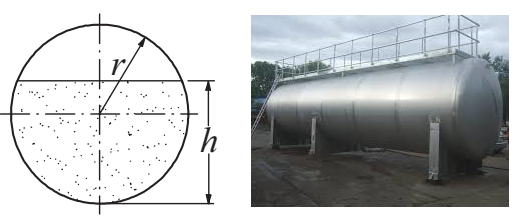
\includegraphics[width=0.7\linewidth]{Figures/oil_tank}
		\caption{Oil tank}
		\label{fig:oiltank}
	\end{figure}
\end{bt}

\begin{bt}(4 điểm) \\
	Cho một cơ cấu tay quay con trượt như trong hình dưới với AB = 0.5m, BC = 1m. Khâu dẫn 1 tạo với phương ngang 1 góc $\phi = $ 45 độ. Xác định vị trí của các khớp $B$, $C$ trong trường hợp này và góc tạo bởi khâu dẫn 2 và phương ngang. 
	Hãy vẽ đồ thị hoành độ $x$ là hàm số thể hiện chuyển động của con trượt $C$ theo góc quay $\phi \in [0,360^o]$.
	\begin{figure}[h!]
		\centering
		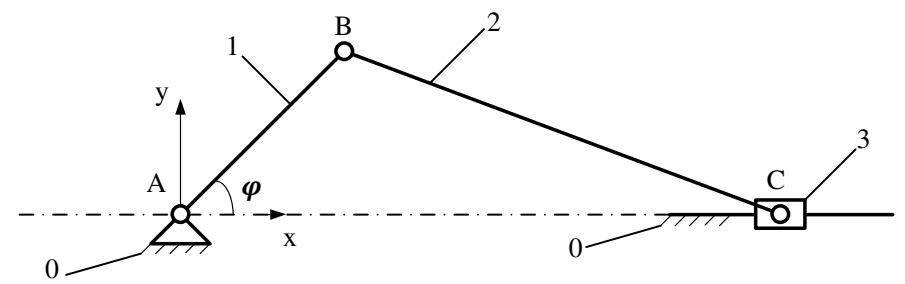
\includegraphics[width=0.7\linewidth]{Figures/tay_quay}
		\caption{Tay quay con trượt}
		\label{fig:tayquay}
	\end{figure}
\end{bt}

\end{document}

\cleardoublepage 

\begin{center}
	{\bf Kiểm tra giữa kỳ - Lý Thuyết - Thời gian 60 phút}
\end{center}
%

\begin{bt}(3 điểm - Chọn 3/5 câu dưới đây) \\
a)	Chứng minh rằng phương trình $1+4x-10x^3=0$ có nghiệm duy nhất trong đoạn $[0.5, 1]$. \\
b)	Để giải phương trình trong câu a), ta xét 2 phép lặp đơn ($x=\varphi(x)$) như sau.
%
\[
i) \ \varphi(x) = 1+5x-10x^3 \ , \hskip 4cm \qquad ii) \ \varphi(x) = \sqrt{\dfrac{1+4x}{10x}} \ .
\]
%
Hãy biện luận về tính hội tụ của các phép lặp trên. \textbf{Trong các câu sau đây ta chỉ xét phép lặp ii).} \\
c) Tìm số bước lặp cần thiết sao cho sai số tuyệt đối của nghiệm bé hơn $1e-6$, cho $x_0 = 0.9$. \\
d) Đưa ra công thức đánh giá ước lượng hậu nghiệm cho $x_3$, bắt đầu từ $x_0 = 0.9$. \\ 
e) Để đạt sai số tuyệt đối $tol = 1e-12$, người ta dự định chọn 2 điều kiện ban đầu $x_0 = 0.9$ và $\tilde{x}_0 = 0.5$. Hãy dự đoán xem với điều kiện ban đầu nào thì cần ít bước lặp hơn để đạt được nghiệm xấp xỉ mong muốn. Giải thích lí do vì sao?
\end{bt}


\begin{bt}(3 điểm)
Cho hàm nội suy dạng $f(x) = \log_{10}(ax^2+bx+c)$ và bảng dữ liệu sau. 
%
\begin{center}
	\begin{tabular}[6]{|l|l|l|l|l|l} \hline
		x & 0 & 1 & 2  & -1   \\ \hline 
		y & -0.1625 & 0.5766 & 1.1346 & -1.1394 \\ \hline
	\end{tabular}	
\end{center}
%
a) Sử dụng phương pháp nội suy Lagrange, tính giá trị $f(1.2)$ chính xác đến 4 chữ số thập phân. \\
b) Sử dụng phương pháp nội suy Newton (lập bảng tỷ sai phân), hãy tính toán chính xác đến 4 chữ số thập phân vector hệ số [a, b, c].
\end{bt}


\begin{bt}(4 điểm) Cường độ bức xạ $\gamma$ của một chất phóng xạ được đo cứ 6 tháng một lần. Kết quả là
%
\begin{center}
	\begin{tabular}[7]{|l|l|l|l|l|} \hline
		t (năm thứ) &  0 & 0.5 & 1 & 1.5 \\ \hline
		$\gamma$ &  1.000 & 0.994 & 0.990 & 0.985  \\ \hline
	\end{tabular}	
\end{center}
%
Biết rằng độ phóng xạ phân rã theo hàm $\gamma(t) = c e^{a t^2 + bt}$, hãy thực hiện các yêu cầu sau. \\
a) Chuyển bài toán về dạng bình phương tối thiểu $\|Ax-b\|_2 \rightarrow \mathrm{min}$. \\
b) Hãy tìm hàm xấp xỉ tốt nhất bảng số liệu sử dụng phương trình chính tắc và phân tích Cholesky, tính toán chính xác đến 3 chữ số thập phân. \\
c) Hãy tìm hàm xấp xỉ tốt nhất sử dụng phương pháp QR, tính toán chính xác đến 3 chữ số thập phân. \textbf{Đáp án chỉ ghi vector hệ số [a, b, c].}
\end{bt}

\end{document}

\begin{center}
\textbf{ Bài tập lập trình.  \ Đề 1. Jacobi + Gauss-Seidel}
\end{center}

\begin{bt}
	Viết 2 hàm trong Python để giải hệ phương trình $Ax=b$ như sau
	%
	\begin{lstlisting}[frame=single] 
	def Jacobi(A,b,nmax,tol):
	return p
	\end{lstlisting}
	%
	và
	%
	\begin{lstlisting}[frame=single] 
	def Gauss_Seidel(A,b,nmax,tol):
	return p
	\end{lstlisting}
	%
	Ở đây nmax là số bước lặp tối đa, tol là sai số cần đạt được giữa nghiệm chính xác và nghiệm xấp xỉ.
	Trong script test luôn cho trường hợp $A =\m{-2 & 5 & 9 \\ 7 & 1 & 1 \\ -3 & 7 & -1}$, $b=\m{1 \\ 6 \\ -26}$ với nmax, tol tùy chọn.
\end{bt}

\begin{bt} % Che/Kincaid 07, page 503, Ex. 16
Sử dụng hai hàm vừa viết trong bài trên để giải hệ phương trình sau với sai số $eps=1e-6$, $nmax=100$.
\begin{equation*}
\m{4 & -1 & 0 & 0 \\ -1 & 4 & -1 & 0 \\ 0 & -1 & 4 & -1 \\ 0 & 0 & -1 & 3} x = \m{15 \\ 10 \\ 10 \\ 10} \ .
\end{equation*}
\end{bt}

\vspace{1cm}
\noindent{\bf Chú ý:} {\it Cán bộ coi thi không giải thích gì thêm}\\


\cleardoublepage 

\begin{center}	
	\textbf{ Đề II} \\
	\textbf{  Bài tập lý thuyết.  \ Đề 2. Newton + Gauss-Seidel }
\end{center}

\begin{bt}(2 điểm) % Exercises 10,11,12, Atkinson/Han p.89
a) Hãy viết công thức lặp trong phương pháp Newton để giải các phương trình sau: \\
\indent i)  $e^x = 4 x $, với $x_0 = 1$, \hskip 4cm \quad 	ii) $x^{1/3} = 0$, với $x_0 = 1$. \\ 
b) Tìm $x_i$, $i=1,...,6$ chính xác đến 4 chữ số thập phân. Biện luận về tính hội tụ của phương pháp Newton trong hai trường hợp trên.
\end{bt}

%\begin{bt}(1 điểm)
%Xét hệ phương trình sau với tham số $\alpha$
%%
%\begin{align*}
%x_1        + \alpha x_2 				&= b_1 \\
%\alpha x_1 + x_2         + \alpha x_3   &= b_2 \\
%             \alpha x_2  + x_3          &= b_3 
%\end{align*}
%%
%Viết công thức lặp Gauss-Seidel cho hệ phương trình trên. Xác định điều kiện của $\alpha$ sao cho phương pháp lặp đó hội tụ sử dụng các chuẩn khác nhau.
%\end{bt}

\begin{bt}(4 điểm)
	a) Viết công thức lặp để giải hệ phương trình sau bằng phương pháp Gauss-Seidel. Phương pháp lặp này có hội tụ không? Vì sao?
	%
	\begin{align*}
	4 x_1 + 0.4 x_2 - 0.4 x_3 &= 8 \\
	0.3 x_1 - 3 x_2 - 0.6 x_3 &= -9 \\
	0.5 x_1 + 0.5 x_2 - 5 x_3 &= 5 
	\end{align*}
	%
	b) Đối với hệ mà các em thu được bằng phương pháp Gauss-Seidel, hãy tìm $\|\cdot\|_1$ và $\|\cdot\|_{\infty}$ của ma trận hệ số vuông cỡ $3 \times 3$. \\
	c) Tính số bước lặp cần thiết bằng ước lượng tiên nghiệm sao cho ta có ước lượng sai số nghiệm $\|x^*-x^n\| \leq 1e-6$, với chuẩn $\|\cdot\|$ phù hợp. \\
	d) Cho $x^0 = \m{0 & 0 & 0}^T$. Hãy tìm $x^i$, $i=1,2,3$. Viết công thức ước lượng hậu nghiệm để đánh giá sai số của $x_3$. \\
	e) Trực chuẩn hóa các vector cột của ma trận bên vế trái, tính toán chính xác đến 3 chữ số thập phân. Từ đó suy ra phân tích QR của ma trận hệ số bên vế trái.
\end{bt}

\cleardoublepage
\begin{center}
	\textbf{  Bài tập lập trình.  \ Đề 2. Curve fitting, phải lập hpt để chuyển về bình phương tối thiểu và giải bằng cả 2 phương pháp.}
\end{center}

\begin{bt}
	Viết 2 hàm trong Python để giải bài toán curve fitting có dạng
	%
	\begin{lstlisting}[frame=single] 
	def curve_fitting_normal_equation(x,y,n):
	return p
	\end{lstlisting}
	%
	bằng phương pháp phương trình chính tắc, và
	%
	\begin{lstlisting}[frame=single] 
	def curve_fitting_qr(x,y,n):
	return p
	\end{lstlisting}
	%
	bằng phương pháp QR. Ở đây, x, y là các vector lưu dữ liệu, n là bậc của đường cong đa thức ($1 \leq n\leq 3$), tức là $y \approx p_0 x^n+p_1 x^{n-1}+...+p_n$. Vector output $p=[p_0 \ p_1 \ ... \ p_n]$.	
	Yêu cầu phải lập hệ phương trình để chuyển về bình phương tối thiểu và giải bằng cả 2 phương pháp. Thầy cho phép gọi trực tiếp các hàm qr và solve trong python.
\end{bt}

Sử dụng hàm vừa viết để giải bài toán sau.

\begin{bt} % Che/Kincaid 07, page 503, Ex. 16
	Độ nhớt của một chất lưu là thông số đại diện cho ma sát trong của dòng chảy. Độ nhớt được biểu diễn qua một hàm bậc hai của nhiệt độ T, tức là $V = a + bT + cT^2$. Hãy tìm hàm xấp xỉ tốt nhất bảng số liệu sau theo phương pháp bình phương tối thiểu.
	%
	\begin{center}
		\begin{tabular}[7]{l|l|l|l|l|l|l|l}
			T & 1    & 2    & 3    & 4    & 5    & 6    & 7 \\ \hline
			V & 2.31 & 2.01 & 1.80 & 1.66 & 1.55 & 1.47 & 1.41.
		\end{tabular}	
	\end{center}
	%
\end{bt}

\centerline{———————————Hết——————————-}


%\end{document}

\vspace{1cm}
\noindent{\bf Chú ý:} {\it Cán bộ coi thi không giải thích gì thêm}\\
\Closesolutionfile{ans}
\newpage
\begin{center}
{\LARGE{\bf ĐÁP ÁN}}
\end{center}

\begin{sol}
Ta có thể xét các phép lặp đơn sau 
\begin{enumerate}
\item[i)] $\varphi(x) = 1+5x-10x^3$ (phân kỳ),
\item[ii)] $\varphi(x) = \cfrac{10x^3-1}{4}$ (phân kỳ),
\item[iii)] $\varphi(x) = \dfrac{1+4x}{10x^2}$ (hội tụ),
\item[iv)] $\varphi(x) = \sqrt{\dfrac{1+4x}{10x}}$ (hội tụ rất nhanh).
\end{enumerate}
%
The best solution would be iv), since the contraction constant on the interval $[0.7,0.8]$ is approximately $0.14$.
\end{sol}
   




